% Options for packages loaded elsewhere
% Options for packages loaded elsewhere
\PassOptionsToPackage{unicode}{hyperref}
\PassOptionsToPackage{hyphens}{url}
\PassOptionsToPackage{dvipsnames,svgnames,x11names}{xcolor}
%
\documentclass[
  11pt]{article}
\usepackage{xcolor}
\usepackage[margin=1in]{geometry}
\usepackage{amsmath,amssymb}
\setcounter{secnumdepth}{-\maxdimen} % remove section numbering
\usepackage{iftex}
\ifPDFTeX
  \usepackage[T1]{fontenc}
  \usepackage[utf8]{inputenc}
  \usepackage{textcomp} % provide euro and other symbols
\else % if luatex or xetex
  \usepackage{unicode-math} % this also loads fontspec
  \defaultfontfeatures{Scale=MatchLowercase}
  \defaultfontfeatures[\rmfamily]{Ligatures=TeX,Scale=1}
\fi
\usepackage{lmodern}
\ifPDFTeX\else
  % xetex/luatex font selection
\fi
% Use upquote if available, for straight quotes in verbatim environments
\IfFileExists{upquote.sty}{\usepackage{upquote}}{}
\IfFileExists{microtype.sty}{% use microtype if available
  \usepackage[]{microtype}
  \UseMicrotypeSet[protrusion]{basicmath} % disable protrusion for tt fonts
}{}
\makeatletter
\@ifundefined{KOMAClassName}{% if non-KOMA class
  \IfFileExists{parskip.sty}{%
    \usepackage{parskip}
  }{% else
    \setlength{\parindent}{0pt}
    \setlength{\parskip}{6pt plus 2pt minus 1pt}}
}{% if KOMA class
  \KOMAoptions{parskip=half}}
\makeatother
% Make \paragraph and \subparagraph free-standing
\makeatletter
\ifx\paragraph\undefined\else
  \let\oldparagraph\paragraph
  \renewcommand{\paragraph}{
    \@ifstar
      \xxxParagraphStar
      \xxxParagraphNoStar
  }
  \newcommand{\xxxParagraphStar}[1]{\oldparagraph*{#1}\mbox{}}
  \newcommand{\xxxParagraphNoStar}[1]{\oldparagraph{#1}\mbox{}}
\fi
\ifx\subparagraph\undefined\else
  \let\oldsubparagraph\subparagraph
  \renewcommand{\subparagraph}{
    \@ifstar
      \xxxSubParagraphStar
      \xxxSubParagraphNoStar
  }
  \newcommand{\xxxSubParagraphStar}[1]{\oldsubparagraph*{#1}\mbox{}}
  \newcommand{\xxxSubParagraphNoStar}[1]{\oldsubparagraph{#1}\mbox{}}
\fi
\makeatother

\usepackage{color}
\usepackage{fancyvrb}
\newcommand{\VerbBar}{|}
\newcommand{\VERB}{\Verb[commandchars=\\\{\}]}
\DefineVerbatimEnvironment{Highlighting}{Verbatim}{commandchars=\\\{\}}
% Add ',fontsize=\small' for more characters per line
\usepackage{framed}
\definecolor{shadecolor}{RGB}{241,243,245}
\newenvironment{Shaded}{\begin{snugshade}}{\end{snugshade}}
\newcommand{\AlertTok}[1]{\textcolor[rgb]{0.68,0.00,0.00}{#1}}
\newcommand{\AnnotationTok}[1]{\textcolor[rgb]{0.37,0.37,0.37}{#1}}
\newcommand{\AttributeTok}[1]{\textcolor[rgb]{0.40,0.45,0.13}{#1}}
\newcommand{\BaseNTok}[1]{\textcolor[rgb]{0.68,0.00,0.00}{#1}}
\newcommand{\BuiltInTok}[1]{\textcolor[rgb]{0.00,0.23,0.31}{#1}}
\newcommand{\CharTok}[1]{\textcolor[rgb]{0.13,0.47,0.30}{#1}}
\newcommand{\CommentTok}[1]{\textcolor[rgb]{0.37,0.37,0.37}{#1}}
\newcommand{\CommentVarTok}[1]{\textcolor[rgb]{0.37,0.37,0.37}{\textit{#1}}}
\newcommand{\ConstantTok}[1]{\textcolor[rgb]{0.56,0.35,0.01}{#1}}
\newcommand{\ControlFlowTok}[1]{\textcolor[rgb]{0.00,0.23,0.31}{\textbf{#1}}}
\newcommand{\DataTypeTok}[1]{\textcolor[rgb]{0.68,0.00,0.00}{#1}}
\newcommand{\DecValTok}[1]{\textcolor[rgb]{0.68,0.00,0.00}{#1}}
\newcommand{\DocumentationTok}[1]{\textcolor[rgb]{0.37,0.37,0.37}{\textit{#1}}}
\newcommand{\ErrorTok}[1]{\textcolor[rgb]{0.68,0.00,0.00}{#1}}
\newcommand{\ExtensionTok}[1]{\textcolor[rgb]{0.00,0.23,0.31}{#1}}
\newcommand{\FloatTok}[1]{\textcolor[rgb]{0.68,0.00,0.00}{#1}}
\newcommand{\FunctionTok}[1]{\textcolor[rgb]{0.28,0.35,0.67}{#1}}
\newcommand{\ImportTok}[1]{\textcolor[rgb]{0.00,0.46,0.62}{#1}}
\newcommand{\InformationTok}[1]{\textcolor[rgb]{0.37,0.37,0.37}{#1}}
\newcommand{\KeywordTok}[1]{\textcolor[rgb]{0.00,0.23,0.31}{\textbf{#1}}}
\newcommand{\NormalTok}[1]{\textcolor[rgb]{0.00,0.23,0.31}{#1}}
\newcommand{\OperatorTok}[1]{\textcolor[rgb]{0.37,0.37,0.37}{#1}}
\newcommand{\OtherTok}[1]{\textcolor[rgb]{0.00,0.23,0.31}{#1}}
\newcommand{\PreprocessorTok}[1]{\textcolor[rgb]{0.68,0.00,0.00}{#1}}
\newcommand{\RegionMarkerTok}[1]{\textcolor[rgb]{0.00,0.23,0.31}{#1}}
\newcommand{\SpecialCharTok}[1]{\textcolor[rgb]{0.37,0.37,0.37}{#1}}
\newcommand{\SpecialStringTok}[1]{\textcolor[rgb]{0.13,0.47,0.30}{#1}}
\newcommand{\StringTok}[1]{\textcolor[rgb]{0.13,0.47,0.30}{#1}}
\newcommand{\VariableTok}[1]{\textcolor[rgb]{0.07,0.07,0.07}{#1}}
\newcommand{\VerbatimStringTok}[1]{\textcolor[rgb]{0.13,0.47,0.30}{#1}}
\newcommand{\WarningTok}[1]{\textcolor[rgb]{0.37,0.37,0.37}{\textit{#1}}}

\usepackage{longtable,booktabs,array}
\usepackage{calc} % for calculating minipage widths
% Correct order of tables after \paragraph or \subparagraph
\usepackage{etoolbox}
\makeatletter
\patchcmd\longtable{\par}{\if@noskipsec\mbox{}\fi\par}{}{}
\makeatother
% Allow footnotes in longtable head/foot
\IfFileExists{footnotehyper.sty}{\usepackage{footnotehyper}}{\usepackage{footnote}}
\makesavenoteenv{longtable}
\usepackage{graphicx}
\makeatletter
\newsavebox\pandoc@box
\newcommand*\pandocbounded[1]{% scales image to fit in text height/width
  \sbox\pandoc@box{#1}%
  \Gscale@div\@tempa{\textheight}{\dimexpr\ht\pandoc@box+\dp\pandoc@box\relax}%
  \Gscale@div\@tempb{\linewidth}{\wd\pandoc@box}%
  \ifdim\@tempb\p@<\@tempa\p@\let\@tempa\@tempb\fi% select the smaller of both
  \ifdim\@tempa\p@<\p@\scalebox{\@tempa}{\usebox\pandoc@box}%
  \else\usebox{\pandoc@box}%
  \fi%
}
% Set default figure placement to htbp
\def\fps@figure{htbp}
\makeatother





\setlength{\emergencystretch}{3em} % prevent overfull lines

\providecommand{\tightlist}{%
  \setlength{\itemsep}{0pt}\setlength{\parskip}{0pt}}



 


\usepackage{fancyhdr}
\usepackage{setspace}
\onehalfspacing
\pagestyle{fancy}
\lhead{DATA 621}
\rhead{Naomi Buell, Richie Rivera, Alexander Simon, Nana Frimpong, Said Naqwe}
\setcounter{secnumdepth}{7}
\makeatletter
\@ifpackageloaded{tcolorbox}{}{\usepackage[skins,breakable]{tcolorbox}}
\@ifpackageloaded{fontawesome5}{}{\usepackage{fontawesome5}}
\definecolor{quarto-callout-color}{HTML}{909090}
\definecolor{quarto-callout-note-color}{HTML}{0758E5}
\definecolor{quarto-callout-important-color}{HTML}{CC1914}
\definecolor{quarto-callout-warning-color}{HTML}{EB9113}
\definecolor{quarto-callout-tip-color}{HTML}{00A047}
\definecolor{quarto-callout-caution-color}{HTML}{FC5300}
\definecolor{quarto-callout-color-frame}{HTML}{acacac}
\definecolor{quarto-callout-note-color-frame}{HTML}{4582ec}
\definecolor{quarto-callout-important-color-frame}{HTML}{d9534f}
\definecolor{quarto-callout-warning-color-frame}{HTML}{f0ad4e}
\definecolor{quarto-callout-tip-color-frame}{HTML}{02b875}
\definecolor{quarto-callout-caution-color-frame}{HTML}{fd7e14}
\makeatother
\makeatletter
\@ifpackageloaded{caption}{}{\usepackage{caption}}
\AtBeginDocument{%
\ifdefined\contentsname
  \renewcommand*\contentsname{Table of contents}
\else
  \newcommand\contentsname{Table of contents}
\fi
\ifdefined\listfigurename
  \renewcommand*\listfigurename{List of Figures}
\else
  \newcommand\listfigurename{List of Figures}
\fi
\ifdefined\listtablename
  \renewcommand*\listtablename{List of Tables}
\else
  \newcommand\listtablename{List of Tables}
\fi
\ifdefined\figurename
  \renewcommand*\figurename{Figure}
\else
  \newcommand\figurename{Figure}
\fi
\ifdefined\tablename
  \renewcommand*\tablename{Table}
\else
  \newcommand\tablename{Table}
\fi
}
\@ifpackageloaded{float}{}{\usepackage{float}}
\floatstyle{ruled}
\@ifundefined{c@chapter}{\newfloat{codelisting}{h}{lop}}{\newfloat{codelisting}{h}{lop}[chapter]}
\floatname{codelisting}{Listing}
\newcommand*\listoflistings{\listof{codelisting}{List of Listings}}
\makeatother
\makeatletter
\makeatother
\makeatletter
\@ifpackageloaded{caption}{}{\usepackage{caption}}
\@ifpackageloaded{subcaption}{}{\usepackage{subcaption}}
\makeatother
\usepackage{bookmark}
\IfFileExists{xurl.sty}{\usepackage{xurl}}{} % add URL line breaks if available
\urlstyle{same}
\hypersetup{
  pdftitle={LOGISTIC REGRESSION},
  pdfauthor={Naomi Buell; Richie Rivera; Alexander Simon; Nana Frimpong; Said Naqwe},
  colorlinks=true,
  linkcolor={blue},
  filecolor={Maroon},
  citecolor={Blue},
  urlcolor={Blue},
  pdfcreator={LaTeX via pandoc}}


\title{LOGISTIC REGRESSION}
\usepackage{etoolbox}
\makeatletter
\providecommand{\subtitle}[1]{% add subtitle to \maketitle
  \apptocmd{\@title}{\par {\large #1 \par}}{}{}
}
\makeatother
\subtitle{Homework \#3}
\author{Naomi Buell \and Richie Rivera \and Alexander Simon \and Nana
Frimpong \and Said Naqwe}
\date{2026-04-12}
\begin{document}
\maketitle


\section{Introduction}\label{introduction}

We build a binary logistic regression model on a data set containing
information on crime for various neighborhoods of a major city to
predict whether the neighborhood will be at risk for high crime levels.
Each record in our data has a response variable indicating whether or
not the crime rate is above the median crime rate or not. Our R
statistical programming code is included in Appendix A.

\section{Data Exploration}\label{data-exploration}

\begin{tcolorbox}[enhanced jigsaw, titlerule=0mm, title=\textcolor{quarto-callout-note-color}{\faInfo}\hspace{0.5em}{Note}, toptitle=1mm, colframe=quarto-callout-note-color-frame, colback=white, coltitle=black, opacityback=0, bottomtitle=1mm, opacitybacktitle=0.6, leftrule=.75mm, rightrule=.15mm, colbacktitle=quarto-callout-note-color!10!white, arc=.35mm, toprule=.15mm, left=2mm, breakable, bottomrule=.15mm]

Data exploration section completed.

\end{tcolorbox}

The crime training data set contains 466 rows and 13 features, and is
100 percent complete. The data are all numeric, and the target variable
is \texttt{target}, which represents whether the crime rate is above the
median crime rate (1) or not (0). The other variables represent various
information on crime for neighborhoods of a major city. See Appendix B
for a full list of variable names and definitions.
Table~\ref{tbl-summary-statistics} presents descriptive characteristics
of the training data.

\begin{longtable}[]{@{}
  >{\raggedright\arraybackslash}p{(\linewidth - 14\tabcolsep) * \real{0.1286}}
  >{\raggedleft\arraybackslash}p{(\linewidth - 14\tabcolsep) * \real{0.2571}}
  >{\raggedleft\arraybackslash}p{(\linewidth - 14\tabcolsep) * \real{0.1143}}
  >{\raggedleft\arraybackslash}p{(\linewidth - 14\tabcolsep) * \real{0.1000}}
  >{\raggedleft\arraybackslash}p{(\linewidth - 14\tabcolsep) * \real{0.1000}}
  >{\raggedleft\arraybackslash}p{(\linewidth - 14\tabcolsep) * \real{0.1000}}
  >{\raggedleft\arraybackslash}p{(\linewidth - 14\tabcolsep) * \real{0.1000}}
  >{\raggedleft\arraybackslash}p{(\linewidth - 14\tabcolsep) * \real{0.1000}}@{}}

\caption{\label{tbl-summary-statistics}Summary statistics for all
variables in the training dataset}

\tabularnewline

\toprule\noalign{}
\begin{minipage}[b]{\linewidth}\raggedright
Variable
\end{minipage} & \begin{minipage}[b]{\linewidth}\raggedleft
Completeness rate
\end{minipage} & \begin{minipage}[b]{\linewidth}\raggedleft
Mean
\end{minipage} & \begin{minipage}[b]{\linewidth}\raggedleft
Min
\end{minipage} & \begin{minipage}[b]{\linewidth}\raggedleft
P25
\end{minipage} & \begin{minipage}[b]{\linewidth}\raggedleft
P50
\end{minipage} & \begin{minipage}[b]{\linewidth}\raggedleft
P75
\end{minipage} & \begin{minipage}[b]{\linewidth}\raggedleft
Max
\end{minipage} \\
\midrule\noalign{}
\endhead
\bottomrule\noalign{}
\endlastfoot
zn & 1 & 12.000 & 0.00 & 0.00 & 0.00 & 16.00 & 100.00 \\
indus & 1 & 11.000 & 0.46 & 5.10 & 9.70 & 18.00 & 28.00 \\
chas & 1 & 0.071 & 0.00 & 0.00 & 0.00 & 0.00 & 1.00 \\
nox & 1 & 0.550 & 0.39 & 0.45 & 0.54 & 0.62 & 0.87 \\
rm & 1 & 6.300 & 3.90 & 5.90 & 6.20 & 6.60 & 8.80 \\
age & 1 & 68.000 & 2.90 & 44.00 & 77.00 & 94.00 & 100.00 \\
dis & 1 & 3.800 & 1.10 & 2.10 & 3.20 & 5.20 & 12.00 \\
rad & 1 & 9.500 & 1.00 & 4.00 & 5.00 & 24.00 & 24.00 \\
tax & 1 & 410.000 & 190.00 & 280.00 & 330.00 & 670.00 & 710.00 \\
ptratio & 1 & 18.000 & 13.00 & 17.00 & 19.00 & 20.00 & 22.00 \\
lstat & 1 & 13.000 & 1.70 & 7.00 & 11.00 & 17.00 & 38.00 \\
medv & 1 & 23.000 & 5.00 & 17.00 & 21.00 & 25.00 & 50.00 \\
target & 1 & 0.490 & 0.00 & 0.00 & 0.00 & 1.00 & 1.00 \\

\end{longtable}

\begin{figure}

\centering{

\pandocbounded{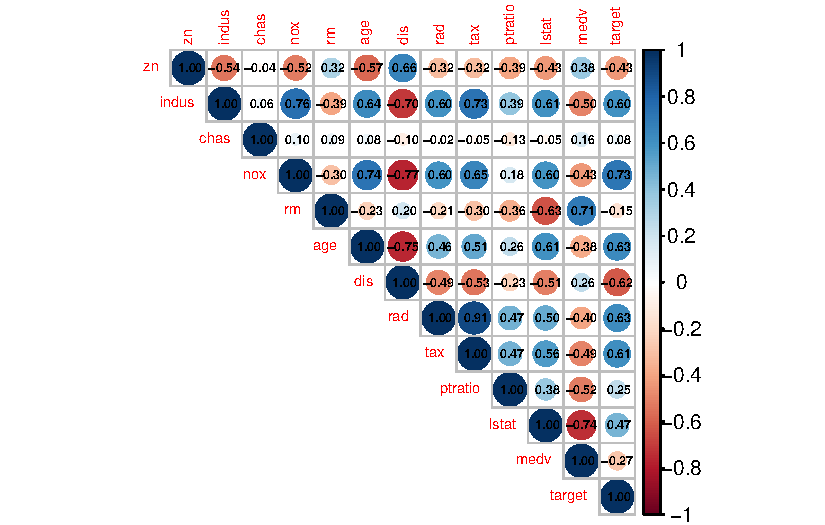
\includegraphics[keepaspectratio]{HW-3_files/figure-pdf/fig-correlation-matrix-1.pdf}}

}

\caption{\label{fig-correlation-matrix}Correlation matrix of all
variables in the training dataset}

\end{figure}%

The correlation between all variables are shown
Figure~\ref{fig-correlation-matrix}. The most correlated predictor
variables with \texttt{target} are \texttt{nox} (nitrogen oxides
concentration, R = 0.73), \texttt{age} (proportion of owner-occupied
units built prior to 1940, R = 0.63), \texttt{rad} (index of
accessibility to radial highways, R = 0.63), \texttt{dis} (weighted mean
of distances to five Boston employment centers, R = -0.62), \texttt{tax}
(full-value property-tax rate per \$10,000, R = 0.61), and
\texttt{indus} (proportion of non-retail business acres per suburb, R =
0.6). These variables have the strongest linear relationships with the
target variable and may be good predictors of crime rates.

\begin{longtable}[]{@{}llr@{}}

\caption{\label{tbl-most-correlated-predictors}Multicollinear variables
in the training dataset}

\tabularnewline

\toprule\noalign{}
Predictor 1 & Predictor 2 & Correlation \\
\midrule\noalign{}
\endhead
\bottomrule\noalign{}
\endlastfoot
rad & tax & 0.91 \\
nox & dis & -0.77 \\
indus & nox & 0.76 \\
age & dis & -0.75 \\
lstat & medv & -0.74 \\
nox & age & 0.74 \\
indus & tax & 0.73 \\
nox & target & 0.73 \\
rm & medv & 0.71 \\
indus & dis & -0.70 \\

\end{longtable}

Table~\ref{tbl-most-correlated-predictors} shows predictor pairs with a
pairwise correlation coefficient greater than 0.7. High pairwise
correlation can create modeling issues because it becomes harder to
isolate each predictor's individual effect on the target variable. The
strongest multicollinear pair is \texttt{rad} (accessibility to
highways) and \texttt{tax} (property-tax rate), which is plausible
because neighborhoods with better highway access may also have higher
property taxes. For this pair, and for the other pairs in the table, we
should consider dropping one variable or using regularization techniques
to mitigate multicollinearity.

\begin{figure}

\centering{

\pandocbounded{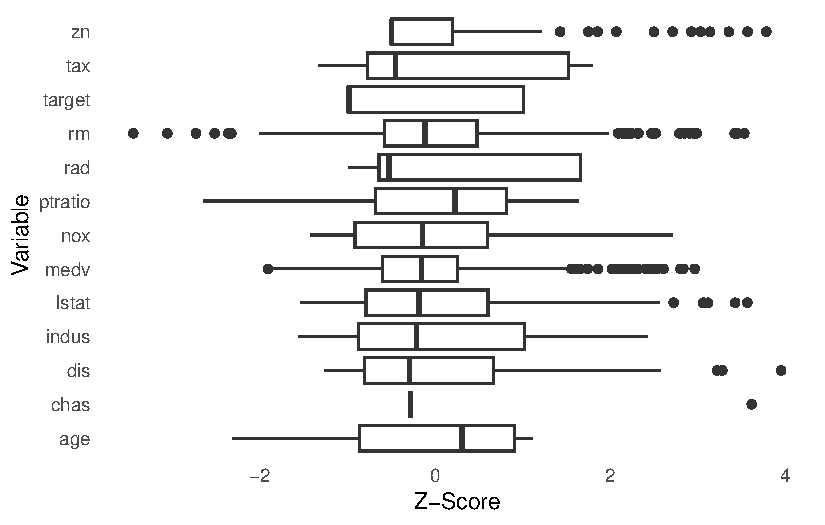
\includegraphics[keepaspectratio]{HW-3_files/figure-pdf/fig-box-plots-1.pdf}}

}

\caption{\label{fig-box-plots}Box plots for identifying outliers in the
training data}

\end{figure}%

Figure~\ref{fig-box-plots} shows the distribution of z-scores for all
variables and highlights potential outliers in the training data. The
variable \texttt{zn} (proportion of residential land zoned for large
lots over 25,000 square feet) has many high outliers, which is plausible
because some neighborhoods may have much higher shares of large lots
than others; its maximum value is 100 percent. The variable \texttt{rm}
(average number of rooms per dwelling) also has several outliers,
ranging from 3.863 to 8.78 rooms. Likewise, \texttt{medv} (median value
of owner-occupied homes) ranges from \$5k to \$50k, which is not
unexpected given variation in housing prices across neighborhoods and
unspecified data years. The variables \texttt{lstat} (percent lower
status population) and \texttt{dis} (weighted mean distance to five
Boston employment centers) show a few high outliers (37.97 percent and
12.1265 units, respectively). The variable \texttt{chas} has a high
value of 1, which is expected because it is a binary indicator of
whether a suburb borders the Charles River. Overall, these outliers
appear to reflect real neighborhood variability rather than data-entry
errors. If influence diagnostics later reveal problematic leverage
points, we can consider adding indicator variables to account for them.

\section{Data Preparation}\label{data-preparation}

\begin{tcolorbox}[enhanced jigsaw, titlerule=0mm, title=\textcolor{quarto-callout-note-color}{\faInfo}\hspace{0.5em}{Note}, toptitle=1mm, colframe=quarto-callout-note-color-frame, colback=white, coltitle=black, opacityback=0, bottomtitle=1mm, opacitybacktitle=0.6, leftrule=.75mm, rightrule=.15mm, colbacktitle=quarto-callout-note-color!10!white, arc=.35mm, toprule=.15mm, left=2mm, breakable, bottomrule=.15mm]

Completed

I don't think we need to compare this dataset to the baseball dataset
(Homework 1).

\end{tcolorbox}

For the crime data used in Homework 3, the first step in data
preparation was to check whether any variables contained missing values.
This crime data set does not contain missing values in either the
training or evaluation files. Therefore, no imputation or missingness
flag variables were needed.

Even though missing-value treatment was unnecessary, we still prepared
the data for binary logistic regression by creating transformed and
derived predictors. Several predictors are right-skewed, especially
\texttt{zn}, \texttt{dis}, \texttt{rad}, \texttt{tax}, and
\texttt{lstat}. For these variables, log transformations were created
using \texttt{log1p()}, which reduces skewness while safely handling
zero values. These transformed variables may improve model fit by making
relationships with the log-odds of the response more stable.

We also created a small set of engineered variables that may be useful
in later models. First, \texttt{nox\_indus} captures the combined effect
of air pollution concentration and industrial land use. Second,
\texttt{rm\_lstat\_ratio} measures the balance between average rooms per
dwelling and lower-status population, combining a housing-quality
measure with a socioeconomic measure. Third, \texttt{tax\_rad\_ratio}
captures the relationship between tax burden and highway accessibility.
These new variables were created because logistic regression can benefit
from transformed and combined predictors when the original variables may
not fully capture the structure related to high-crime neighborhoods.

Finally, the cleaned training and evaluation data sets were stored as
\texttt{crime\_clean} and \texttt{crime\_eval\_clean} so the later
modeling section can use them directly.

\begin{Shaded}
\begin{Highlighting}[]
\CommentTok{\# Check missing values in training and evaluation data}
\NormalTok{missing\_train }\OtherTok{\textless{}{-}}\NormalTok{ crime\_train }\SpecialCharTok{|\textgreater{}}
  \FunctionTok{summarise}\NormalTok{(}\FunctionTok{across}\NormalTok{(}\FunctionTok{everything}\NormalTok{(), }\SpecialCharTok{\textasciitilde{}} \FunctionTok{sum}\NormalTok{(}\FunctionTok{is.na}\NormalTok{(.)))) }\SpecialCharTok{|\textgreater{}}
  \FunctionTok{pivot\_longer}\NormalTok{(}\FunctionTok{everything}\NormalTok{(), }\AttributeTok{names\_to =} \StringTok{"Variable"}\NormalTok{, }\AttributeTok{values\_to =} \StringTok{"Missing"}\NormalTok{)}

\NormalTok{missing\_eval }\OtherTok{\textless{}{-}}\NormalTok{ crime\_eval }\SpecialCharTok{|\textgreater{}}
  \FunctionTok{summarise}\NormalTok{(}\FunctionTok{across}\NormalTok{(}\FunctionTok{everything}\NormalTok{(), }\SpecialCharTok{\textasciitilde{}} \FunctionTok{sum}\NormalTok{(}\FunctionTok{is.na}\NormalTok{(.)))) }\SpecialCharTok{|\textgreater{}}
  \FunctionTok{pivot\_longer}\NormalTok{(}\FunctionTok{everything}\NormalTok{(), }\AttributeTok{names\_to =} \StringTok{"Variable"}\NormalTok{, }\AttributeTok{values\_to =} \StringTok{"Missing"}\NormalTok{)}

\NormalTok{missing\_train}
\end{Highlighting}
\end{Shaded}

\begin{verbatim}
# A tibble: 13 x 2
   Variable Missing
   <chr>      <int>
 1 zn             0
 2 indus          0
 3 chas           0
 4 nox            0
 5 rm             0
 6 age            0
 7 dis            0
 8 rad            0
 9 tax            0
10 ptratio        0
11 lstat          0
12 medv           0
13 target         0
\end{verbatim}

\begin{Shaded}
\begin{Highlighting}[]
\NormalTok{missing\_eval}
\end{Highlighting}
\end{Shaded}

\begin{verbatim}
# A tibble: 12 x 2
   Variable Missing
   <chr>      <int>
 1 zn             0
 2 indus          0
 3 chas           0
 4 nox            0
 5 rm             0
 6 age            0
 7 dis            0
 8 rad            0
 9 tax            0
10 ptratio        0
11 lstat          0
12 medv           0
\end{verbatim}

\begin{Shaded}
\begin{Highlighting}[]
\CommentTok{\#| label: data{-}preparation{-}transformations}
\CommentTok{\#| echo: true}
\CommentTok{\#| warning: false}

\CommentTok{\# Start with copies of the original datasets}
\NormalTok{crime\_clean }\OtherTok{\textless{}{-}}\NormalTok{ crime\_train}
\NormalTok{crime\_eval\_clean }\OtherTok{\textless{}{-}}\NormalTok{ crime\_eval}

\CommentTok{\# Create transformed and engineered predictors}
\NormalTok{crime\_clean }\OtherTok{\textless{}{-}}\NormalTok{ crime\_clean }\SpecialCharTok{|\textgreater{}}
  \FunctionTok{mutate}\NormalTok{(}
    \CommentTok{\# Log transforms for right{-}skewed predictors}
    \AttributeTok{log\_zn    =} \FunctionTok{log1p}\NormalTok{(zn),}
    \AttributeTok{log\_dis   =} \FunctionTok{log1p}\NormalTok{(dis),}
    \AttributeTok{log\_rad   =} \FunctionTok{log1p}\NormalTok{(rad),}
    \AttributeTok{log\_tax   =} \FunctionTok{log1p}\NormalTok{(tax),}
    \AttributeTok{log\_lstat =} \FunctionTok{log1p}\NormalTok{(lstat),}

    \CommentTok{\# Engineered variables}
    \AttributeTok{nox\_indus     =}\NormalTok{ nox }\SpecialCharTok{*}\NormalTok{ indus,}
    \AttributeTok{rm\_lstat\_ratio =}\NormalTok{ rm }\SpecialCharTok{/}\NormalTok{ lstat,}
    \AttributeTok{tax\_rad\_ratio  =}\NormalTok{ tax }\SpecialCharTok{/}\NormalTok{ rad}
\NormalTok{  )}

\NormalTok{crime\_eval\_clean }\OtherTok{\textless{}{-}}\NormalTok{ crime\_eval\_clean }\SpecialCharTok{|\textgreater{}}
  \FunctionTok{mutate}\NormalTok{(}
    \CommentTok{\# Log transforms for right{-}skewed predictors}
    \AttributeTok{log\_zn    =} \FunctionTok{log1p}\NormalTok{(zn),}
    \AttributeTok{log\_dis   =} \FunctionTok{log1p}\NormalTok{(dis),}
    \AttributeTok{log\_rad   =} \FunctionTok{log1p}\NormalTok{(rad),}
    \AttributeTok{log\_tax   =} \FunctionTok{log1p}\NormalTok{(tax),}
    \AttributeTok{log\_lstat =} \FunctionTok{log1p}\NormalTok{(lstat),}

    \CommentTok{\# Engineered variables}
    \AttributeTok{nox\_indus     =}\NormalTok{ nox }\SpecialCharTok{*}\NormalTok{ indus,}
    \AttributeTok{rm\_lstat\_ratio =}\NormalTok{ rm }\SpecialCharTok{/}\NormalTok{ lstat,}
    \AttributeTok{tax\_rad\_ratio  =}\NormalTok{ tax }\SpecialCharTok{/}\NormalTok{ rad}
\NormalTok{  )}

\CommentTok{\#| label: data{-}preparation{-}verify}
\CommentTok{\#| echo: true}

\CommentTok{\# Verify dimensions after preparation}
\FunctionTok{dim}\NormalTok{(crime\_clean)}
\end{Highlighting}
\end{Shaded}

\begin{verbatim}
[1] 466  21
\end{verbatim}

\begin{Shaded}
\begin{Highlighting}[]
\FunctionTok{dim}\NormalTok{(crime\_eval\_clean)}
\end{Highlighting}
\end{Shaded}

\begin{verbatim}
[1] 40 20
\end{verbatim}

\begin{Shaded}
\begin{Highlighting}[]
\CommentTok{\# Verify that no missing values remain after transformations}
\NormalTok{crime\_clean }\SpecialCharTok{|\textgreater{}}
  \FunctionTok{summarise}\NormalTok{(}\FunctionTok{across}\NormalTok{(}\FunctionTok{everything}\NormalTok{(), }\SpecialCharTok{\textasciitilde{}} \FunctionTok{sum}\NormalTok{(}\FunctionTok{is.na}\NormalTok{(.)))) }\SpecialCharTok{|\textgreater{}}
  \FunctionTok{pivot\_longer}\NormalTok{(}\FunctionTok{everything}\NormalTok{(), }\AttributeTok{names\_to =} \StringTok{"Variable"}\NormalTok{, }\AttributeTok{values\_to =} \StringTok{"Missing"}\NormalTok{) }\SpecialCharTok{|\textgreater{}}
  \FunctionTok{filter}\NormalTok{(Missing }\SpecialCharTok{\textgreater{}} \DecValTok{0}\NormalTok{)}
\end{Highlighting}
\end{Shaded}

\begin{verbatim}
# A tibble: 0 x 2
# i 2 variables: Variable <chr>, Missing <int>
\end{verbatim}

\begin{Shaded}
\begin{Highlighting}[]
\NormalTok{crime\_eval\_clean }\SpecialCharTok{|\textgreater{}}
  \FunctionTok{summarise}\NormalTok{(}\FunctionTok{across}\NormalTok{(}\FunctionTok{everything}\NormalTok{(), }\SpecialCharTok{\textasciitilde{}} \FunctionTok{sum}\NormalTok{(}\FunctionTok{is.na}\NormalTok{(.)))) }\SpecialCharTok{|\textgreater{}}
  \FunctionTok{pivot\_longer}\NormalTok{(}\FunctionTok{everything}\NormalTok{(), }\AttributeTok{names\_to =} \StringTok{"Variable"}\NormalTok{, }\AttributeTok{values\_to =} \StringTok{"Missing"}\NormalTok{) }\SpecialCharTok{|\textgreater{}}
  \FunctionTok{filter}\NormalTok{(Missing }\SpecialCharTok{\textgreater{}} \DecValTok{0}\NormalTok{)}
\end{Highlighting}
\end{Shaded}

\begin{verbatim}
# A tibble: 0 x 2
# i 2 variables: Variable <chr>, Missing <int>
\end{verbatim}

\begin{Shaded}
\begin{Highlighting}[]
\DocumentationTok{\#\#\# Linearity Assumption Summary}

\CommentTok{\# The results above indicate that the assumption of linearity is satisfied for all independent variables. However, several were flagged as being unlikely to have predictive value in a multivariate linear model.}

\DocumentationTok{\#\# Data Splits}

\CommentTok{\# First, we will split our dataset into a training and testing set. We will use the training set to build our models and the testing set to evaluate their performance. The training set will be used to fit the models, while the testing set will be used to assess how well the models generalize to new data.}

\CommentTok{\#| label: split{-}data}
\CommentTok{\#| eval: false}

\FunctionTok{set.seed}\NormalTok{(}\DecValTok{19940211}\NormalTok{)}
\NormalTok{train\_indices }\OtherTok{\textless{}{-}} \FunctionTok{sample}\NormalTok{(}\FunctionTok{nrow}\NormalTok{(crime\_clean), }\AttributeTok{size =} \FloatTok{0.8} \SpecialCharTok{*} \FunctionTok{nrow}\NormalTok{(crime\_clean))}
\NormalTok{crime\_train\_split }\OtherTok{\textless{}{-}}\NormalTok{ crime\_clean[train\_indices, ]}
\NormalTok{crime\_test\_split }\OtherTok{\textless{}{-}}\NormalTok{ crime\_clean[}\SpecialCharTok{{-}}\NormalTok{train\_indices, ]}
\end{Highlighting}
\end{Shaded}

\section{Check assumptions for binary logistic
regression}\label{check-assumptions-for-binary-logistic-regression}

\begin{tcolorbox}[enhanced jigsaw, titlerule=0mm, title=\textcolor{quarto-callout-note-color}{\faInfo}\hspace{0.5em}{Note}, toptitle=1mm, colframe=quarto-callout-note-color-frame, colback=white, coltitle=black, opacityback=0, bottomtitle=1mm, opacitybacktitle=0.6, leftrule=.75mm, rightrule=.15mm, colbacktitle=quarto-callout-note-color!10!white, arc=.35mm, toprule=.15mm, left=2mm, breakable, bottomrule=.15mm]

To be added

\end{tcolorbox}

\section{Build models}\label{build-models}

\begin{tcolorbox}[enhanced jigsaw, titlerule=0mm, title=\textcolor{quarto-callout-note-color}{\faInfo}\hspace{0.5em}{Note}, toptitle=1mm, colframe=quarto-callout-note-color-frame, colback=white, coltitle=black, opacityback=0, bottomtitle=1mm, opacitybacktitle=0.6, leftrule=.75mm, rightrule=.15mm, colbacktitle=quarto-callout-note-color!10!white, arc=.35mm, toprule=.15mm, left=2mm, breakable, bottomrule=.15mm]

Completed but file won't render. The rendering fails on line 265, but
I'm not sure what's wrong. Any ideas?

\end{tcolorbox}

We compared three models. Our first model included all the variables in
the cleaned training dataset. The second model aimed to reduce
multicollinearity by omitting variables that had correlation
coefficients \(|r|>0.7\) (see Data Exploration section). Finally, we
generated the third model using backward stepwise selection from a full
model that included transformed variables and newly created variables
(see Data Preparation section).

\subsection{Model 1. All untransformed
variables}\label{model-1.-all-untransformed-variables}

As shown below, the most significant predictors were \texttt{nox} and
\texttt{rad} (\(P<0.001\)). In addition, \texttt{age} and
\texttt{ptratio} were significant at the \(P<0.01\) level, and
\texttt{dis} and \texttt{tax} were significant at the \(P<0.05\) level.
The AIC for this model is \texttt{r\textbackslash{}\ AIC(model1)}.

\begin{Shaded}
\begin{Highlighting}[]
\NormalTok{model1 }\OtherTok{\textless{}{-}} \FunctionTok{glm}\NormalTok{(}
  \AttributeTok{formula =}\NormalTok{ target }\SpecialCharTok{\textasciitilde{}}\NormalTok{ zn }\SpecialCharTok{+}\NormalTok{ indus }\SpecialCharTok{+}\NormalTok{ chas }\SpecialCharTok{+}\NormalTok{ nox }\SpecialCharTok{+}\NormalTok{ rm }\SpecialCharTok{+}\NormalTok{ age }\SpecialCharTok{+}\NormalTok{ dis }\SpecialCharTok{+}\NormalTok{ rad }\SpecialCharTok{+}\NormalTok{ tax }\SpecialCharTok{+}
\NormalTok{                     ptratio }\SpecialCharTok{+}\NormalTok{ lstat }\SpecialCharTok{+}\NormalTok{ medv,}
  \AttributeTok{family =} \StringTok{"binomial"}\NormalTok{,}
  \AttributeTok{data =}\NormalTok{ crime\_train\_split)}

\FunctionTok{summary}\NormalTok{(model1)}
\end{Highlighting}
\end{Shaded}

\begin{verbatim}

Call:
glm(formula = target ~ zn + indus + chas + nox + rm + age + dis + 
    rad + tax + ptratio + lstat + medv, family = "binomial", 
    data = crime_train_split)

Coefficients:
              Estimate Std. Error z value Pr(>|z|)    
(Intercept) -47.929725   8.808610  -5.441 5.29e-08 ***
zn           -0.048895   0.037182  -1.315  0.18851    
indus        -0.054428   0.066155  -0.823  0.41065    
chas          0.924573   1.061844   0.871  0.38390    
nox          55.009200  10.291959   5.345 9.05e-08 ***
rm            0.050251   0.882349   0.057  0.95458    
age           0.048050   0.017874   2.688  0.00718 ** 
dis           0.657857   0.260376   2.527  0.01152 *  
rad           0.783482   0.201429   3.890  0.00010 ***
tax          -0.010043   0.004025  -2.495  0.01259 *  
ptratio       0.475152   0.159502   2.979  0.00289 ** 
lstat         0.010310   0.069436   0.148  0.88196    
medv          0.127463   0.078800   1.618  0.10576    
---
Signif. codes:  0 '***' 0.001 '**' 0.01 '*' 0.05 '.' 0.1 ' ' 1

(Dispersion parameter for binomial family taken to be 1)

    Null deviance: 515.31  on 371  degrees of freedom
Residual deviance: 133.42  on 359  degrees of freedom
AIC: 159.42

Number of Fisher Scoring iterations: 9
\end{verbatim}

\subsection{Model 2. Reduce
multicollinearity}\label{model-2.-reduce-multicollinearity}

In the Data Exploration section, we showed that \texttt{rad} and
\texttt{tax} were strongly correlated (r=0.91), which suggests that only
one of these variables is needed in Model 1 (we chose to retain
\texttt{rad} as it was more highly significant). Similarly,
\texttt{medv} was shown to be potentially multicollinear with
\texttt{lstat} (r=0.74) and \texttt{rm} (r=0.71), so we removed the
latter variables.

In addition, the correlation between \texttt{nox} (predictor) and
\texttt{target} (response) suggests that \texttt{nox} is an important
predictor, so we removed its potential collinear pairs \texttt{age} and
\texttt{dis}. Although \texttt{nox} was moderately correlated with
\texttt{indus} (r=0.76), we retained \texttt{indus} because removal of
both \texttt{indus} and \texttt{tax} (highly correlated with
\texttt{rad}) would eliminate a potentially informative predictor.

These changes resulted in a model with AIC
\texttt{r\textbackslash{}\ AIC(model2)}.

\begin{Shaded}
\begin{Highlighting}[]
\NormalTok{model2 }\OtherTok{\textless{}{-}} \FunctionTok{glm}\NormalTok{(}
  \AttributeTok{formula =}\NormalTok{ target }\SpecialCharTok{\textasciitilde{}}\NormalTok{ zn }\SpecialCharTok{+}\NormalTok{ indus }\SpecialCharTok{+}\NormalTok{ chas }\SpecialCharTok{+}\NormalTok{ nox }\SpecialCharTok{+}\NormalTok{ rad }\SpecialCharTok{+}\NormalTok{ ptratio }\SpecialCharTok{+}\NormalTok{ medv,}
  \AttributeTok{family =} \StringTok{"binomial"}\NormalTok{,}
  \AttributeTok{data =}\NormalTok{ crime\_train\_split)}

\FunctionTok{summary}\NormalTok{(model2)}
\end{Highlighting}
\end{Shaded}

\begin{verbatim}

Call:
glm(formula = target ~ zn + indus + chas + nox + rad + ptratio + 
    medv, family = "binomial", data = crime_train_split)

Coefficients:
             Estimate Std. Error z value Pr(>|z|)    
(Intercept) -34.11942    6.07656  -5.615 1.97e-08 ***
zn           -0.03024    0.02862  -1.057 0.290641    
indus        -0.15005    0.05644  -2.658 0.007851 ** 
chas          1.45828    0.89598   1.628 0.103614    
nox          45.57838    8.64114   5.275 1.33e-07 ***
rad           0.46600    0.14094   3.306 0.000946 ***
ptratio       0.35450    0.13212   2.683 0.007291 ** 
medv          0.08292    0.03159   2.625 0.008656 ** 
---
Signif. codes:  0 '***' 0.001 '**' 0.01 '*' 0.05 '.' 0.1 ' ' 1

(Dispersion parameter for binomial family taken to be 1)

    Null deviance: 515.31  on 371  degrees of freedom
Residual deviance: 157.41  on 364  degrees of freedom
AIC: 173.41

Number of Fisher Scoring iterations: 9
\end{verbatim}

\subsection{Model 3. Backward stepwise variable
selection}\label{model-3.-backward-stepwise-variable-selection}

For this model, we performed backward stepwise selection from the set of
variables including transformed and newly created variables.

The best model had \texttt{nox}, \texttt{tax\_rad\_ratio},
\texttt{ptratio}, and \texttt{age} as the most significant predictors
(P\textless0.001). In addition, \texttt{log\_dis} and
\texttt{rm\_lstat\_ratio} were significant at the P\textless0.05 level.
The AIC of this model was \texttt{r\textbackslash{}\ AIC(model3)}, which
was lower than that of Models 1 and 2.

\begin{Shaded}
\begin{Highlighting}[]
\CommentTok{\# Full model includes all variables}
\NormalTok{model\_full }\OtherTok{\textless{}{-}} \FunctionTok{glm}\NormalTok{(}
  \AttributeTok{formula =}\NormalTok{ target }\SpecialCharTok{\textasciitilde{}}\NormalTok{ log\_zn }\SpecialCharTok{+}\NormalTok{ indus }\SpecialCharTok{+}\NormalTok{ chas }\SpecialCharTok{+}\NormalTok{ nox }\SpecialCharTok{+}\NormalTok{ rm }\SpecialCharTok{+}\NormalTok{ age }\SpecialCharTok{+} 
\NormalTok{                     log\_dis }\SpecialCharTok{+}\NormalTok{ log\_rad }\SpecialCharTok{+}\NormalTok{ log\_tax }\SpecialCharTok{+}\NormalTok{ ptratio }\SpecialCharTok{+}\NormalTok{ log\_lstat }\SpecialCharTok{+}\NormalTok{ medv }\SpecialCharTok{+}
\NormalTok{                     nox\_indus }\SpecialCharTok{+}\NormalTok{ rm\_lstat\_ratio }\SpecialCharTok{+}\NormalTok{ tax\_rad\_ratio,}
  \AttributeTok{family =} \StringTok{"binomial"}\NormalTok{,}
  \AttributeTok{data =}\NormalTok{ crime\_train\_split)}

\CommentTok{\# Select variables}
\NormalTok{model3 }\OtherTok{\textless{}{-}} \FunctionTok{step}\NormalTok{(model\_full, }\AttributeTok{direction =} \StringTok{"backward"}\NormalTok{)}
\end{Highlighting}
\end{Shaded}

\begin{verbatim}
Start:  AIC=158.32
target ~ log_zn + indus + chas + nox + rm + age + log_dis + log_rad + 
    log_tax + ptratio + log_lstat + medv + nox_indus + rm_lstat_ratio + 
    tax_rad_ratio
\end{verbatim}

\begin{verbatim}
Warning: glm.fit: fitted probabilities numerically 0 or 1 occurred
\end{verbatim}

\begin{verbatim}
                 Df Deviance    AIC
- log_tax         1   126.46 156.46
- rm              1   126.47 156.47
- log_zn          1   126.69 156.69
- log_rad         1   127.06 157.06
- log_lstat       1   127.16 157.16
- tax_rad_ratio   1   127.38 157.38
- medv            1   127.45 157.45
- indus           1   127.91 157.91
- chas            1   127.96 157.96
- nox_indus       1   128.02 158.02
<none>                126.32 158.32
- rm_lstat_ratio  1   131.00 161.00
- log_dis         1   132.94 162.94
- age             1   136.32 166.32
- ptratio         1   136.95 166.95
- nox             1   162.12 192.12

Step:  AIC=156.46
target ~ log_zn + indus + chas + nox + rm + age + log_dis + log_rad + 
    ptratio + log_lstat + medv + nox_indus + rm_lstat_ratio + 
    tax_rad_ratio

                 Df Deviance    AIC
- rm              1   126.62 154.62
- log_zn          1   126.82 154.82
- log_lstat       1   127.23 155.23
- medv            1   127.73 155.73
- indus           1   127.92 155.92
- nox_indus       1   128.05 156.05
- log_rad         1   128.31 156.31
- chas            1   128.43 156.43
<none>                126.46 156.46
- rm_lstat_ratio  1   131.03 159.03
- tax_rad_ratio   1   131.18 159.18
- log_dis         1   133.51 161.51
- age             1   136.32 164.32
- ptratio         1   137.07 165.07
- nox             1   166.00 194.00

Step:  AIC=154.62
target ~ log_zn + indus + chas + nox + age + log_dis + log_rad + 
    ptratio + log_lstat + medv + nox_indus + rm_lstat_ratio + 
    tax_rad_ratio

                 Df Deviance    AIC
- log_zn          1   127.11 153.11
- log_lstat       1   127.57 153.57
- indus           1   128.03 154.03
- medv            1   128.13 154.13
- nox_indus       1   128.16 154.16
- log_rad         1   128.31 154.31
- chas            1   128.55 154.55
<none>                126.62 154.62
- rm_lstat_ratio  1   131.04 157.04
- tax_rad_ratio   1   131.58 157.58
- log_dis         1   133.53 159.53
- ptratio         1   137.47 163.47
- age             1   137.57 163.57
- nox             1   166.90 192.90

Step:  AIC=153.11
target ~ indus + chas + nox + age + log_dis + log_rad + ptratio + 
    log_lstat + medv + nox_indus + rm_lstat_ratio + tax_rad_ratio

                 Df Deviance    AIC
- log_lstat       1   127.78 151.78
- medv            1   128.47 152.47
- log_rad         1   128.60 152.60
- indus           1   128.94 152.94
- nox_indus       1   129.06 153.06
<none>                127.11 153.11
- chas            1   129.54 153.54
- rm_lstat_ratio  1   131.31 155.31
- tax_rad_ratio   1   133.10 157.10
- log_dis         1   133.55 157.55
- age             1   138.77 162.77
- ptratio         1   144.07 168.07
- nox             1   170.11 194.11

Step:  AIC=151.78
target ~ indus + chas + nox + age + log_dis + log_rad + ptratio + 
    medv + nox_indus + rm_lstat_ratio + tax_rad_ratio

                 Df Deviance    AIC
- medv            1   129.14 151.14
- log_rad         1   129.55 151.55
- indus           1   129.69 151.69
<none>                127.78 151.78
- nox_indus       1   129.80 151.80
- chas            1   130.22 152.22
- rm_lstat_ratio  1   132.54 154.54
- tax_rad_ratio   1   133.46 155.46
- log_dis         1   135.48 157.48
- age             1   143.24 165.24
- ptratio         1   144.43 166.43
- nox             1   171.35 193.35

Step:  AIC=151.14
target ~ indus + chas + nox + age + log_dis + log_rad + ptratio + 
    nox_indus + rm_lstat_ratio + tax_rad_ratio

                 Df Deviance    AIC
- log_rad         1   130.47 150.47
- indus           1   130.74 150.74
- nox_indus       1   130.86 150.86
<none>                129.14 151.14
- chas            1   131.81 151.81
- log_dis         1   135.48 155.48
- tax_rad_ratio   1   136.34 156.34
- age             1   143.85 163.85
- ptratio         1   145.01 165.01
- rm_lstat_ratio  1   150.57 170.57
- nox             1   171.57 191.57

Step:  AIC=150.47
target ~ indus + chas + nox + age + log_dis + ptratio + nox_indus + 
    rm_lstat_ratio + tax_rad_ratio

                 Df Deviance    AIC
- indus           1   132.01 150.01
- nox_indus       1   132.02 150.02
<none>                130.47 150.47
- chas            1   133.15 151.15
- log_dis         1   135.90 153.90
- age             1   145.28 163.28
- ptratio         1   147.07 165.07
- rm_lstat_ratio  1   151.57 169.57
- nox             1   172.02 190.02
- tax_rad_ratio   1   177.44 195.44

Step:  AIC=150.01
target ~ chas + nox + age + log_dis + ptratio + nox_indus + rm_lstat_ratio + 
    tax_rad_ratio

                 Df Deviance    AIC
- nox_indus       1   132.02 148.02
<none>                132.01 150.01
- chas            1   134.98 150.98
- log_dis         1   137.55 153.55
- age             1   146.75 162.75
- ptratio         1   148.26 164.26
- rm_lstat_ratio  1   151.61 167.61
- tax_rad_ratio   1   184.46 200.46
- nox             1   186.02 202.02

Step:  AIC=148.02
target ~ chas + nox + age + log_dis + ptratio + rm_lstat_ratio + 
    tax_rad_ratio

                 Df Deviance    AIC
<none>                132.02 148.02
- chas            1   135.02 149.02
- log_dis         1   137.66 151.66
- age             1   147.04 161.04
- ptratio         1   148.29 162.29
- rm_lstat_ratio  1   151.61 165.61
- tax_rad_ratio   1   189.81 203.81
- nox             1   215.50 229.50
\end{verbatim}

\begin{Shaded}
\begin{Highlighting}[]
\FunctionTok{summary}\NormalTok{(model3)}
\end{Highlighting}
\end{Shaded}

\begin{verbatim}

Call:
glm(formula = target ~ chas + nox + age + log_dis + ptratio + 
    rm_lstat_ratio + tax_rad_ratio, family = "binomial", data = crime_train_split)

Coefficients:
                Estimate Std. Error z value Pr(>|z|)    
(Intercept)    -44.89858    7.47464  -6.007 1.89e-09 ***
chas             1.55357    0.90952   1.708 0.087613 .  
nox             55.23868    8.90173   6.205 5.46e-10 ***
age              0.05359    0.01503   3.565 0.000364 ***
log_dis          2.64074    1.12460   2.348 0.018867 *  
ptratio          0.50438    0.13160   3.833 0.000127 ***
rm_lstat_ratio   2.52680    0.65649   3.849 0.000119 ***
tax_rad_ratio   -0.05751    0.01302  -4.418 9.95e-06 ***
---
Signif. codes:  0 '***' 0.001 '**' 0.01 '*' 0.05 '.' 0.1 ' ' 1

(Dispersion parameter for binomial family taken to be 1)

    Null deviance: 515.31  on 371  degrees of freedom
Residual deviance: 132.02  on 364  degrees of freedom
AIC: 148.02

Number of Fisher Scoring iterations: 8
\end{verbatim}

Of these three models, model 3 has the lowest AIC. In the next section,
we will evaluate the performance of these models to more determine which
one is best for predicting the \texttt{target} variable.

\section{Select Models}\label{select-models}

\begin{Shaded}
\begin{Highlighting}[]
\CommentTok{\# Creating a custom helper function to extract all the required metrics }
\CommentTok{\# explicitly evaluating on the provided training dataset.}
\NormalTok{get\_model\_metrics }\OtherTok{\textless{}{-}} \ControlFlowTok{function}\NormalTok{(model, model\_name, train\_data) \{}
\NormalTok{  mod\_summary }\OtherTok{\textless{}{-}} \FunctionTok{summary}\NormalTok{(model)}
  
  \CommentTok{\# Explicitly calculate Mean Squared Error (MSE) using the training data}
\NormalTok{  predictions }\OtherTok{\textless{}{-}} \FunctionTok{predict}\NormalTok{(model, }\AttributeTok{newdata =}\NormalTok{ train\_data)}
\NormalTok{  mse }\OtherTok{\textless{}{-}} \FunctionTok{mean}\NormalTok{((train\_data}\SpecialCharTok{$}\NormalTok{TARGET\_WINS }\SpecialCharTok{{-}}\NormalTok{ predictions)}\SpecialCharTok{\^{}}\DecValTok{2}\NormalTok{)}
  
  \CommentTok{\# Extract F{-}statistic and calculate its p{-}value (inherent to training data)}
\NormalTok{  f\_stat }\OtherTok{\textless{}{-}}\NormalTok{ mod\_summary}\SpecialCharTok{$}\NormalTok{fstatistic}
\NormalTok{  p\_val }\OtherTok{\textless{}{-}} \ControlFlowTok{if}\NormalTok{ (}\SpecialCharTok{!}\FunctionTok{is.null}\NormalTok{(f\_stat)) \{}
    \FunctionTok{pf}\NormalTok{(f\_stat[}\DecValTok{1}\NormalTok{], f\_stat[}\DecValTok{2}\NormalTok{], f\_stat[}\DecValTok{3}\NormalTok{], }\AttributeTok{lower.tail =} \ConstantTok{FALSE}\NormalTok{)}
\NormalTok{  \} }\ControlFlowTok{else}\NormalTok{ \{}
    \ConstantTok{NA}
\NormalTok{  \}}
  
  \CommentTok{\# Return a nicely formatted row for our table}
  \FunctionTok{tibble}\NormalTok{(}
    \AttributeTok{Model =}\NormalTok{ model\_name,}
    \StringTok{\textasciigrave{}}\AttributeTok{Training MSE}\StringTok{\textasciigrave{}} \OtherTok{=}\NormalTok{ mse,}
    \StringTok{\textasciigrave{}}\AttributeTok{R{-}Squared}\StringTok{\textasciigrave{}} \OtherTok{=}\NormalTok{ mod\_summary}\SpecialCharTok{$}\NormalTok{r.squared,}
    \StringTok{\textasciigrave{}}\AttributeTok{Adj R{-}Squared}\StringTok{\textasciigrave{}} \OtherTok{=}\NormalTok{ mod\_summary}\SpecialCharTok{$}\NormalTok{adj.r.squared,}
    \StringTok{\textasciigrave{}}\AttributeTok{F{-}Statistic}\StringTok{\textasciigrave{}} \OtherTok{=}\NormalTok{ f\_stat[}\DecValTok{1}\NormalTok{],}
    \StringTok{\textasciigrave{}}\AttributeTok{P{-}Value}\StringTok{\textasciigrave{}} \OtherTok{=}\NormalTok{ p\_val,}
    \StringTok{\textasciigrave{}}\AttributeTok{AIC}\StringTok{\textasciigrave{}} \OtherTok{=} \FunctionTok{AIC}\NormalTok{(model),}
    \StringTok{\textasciigrave{}}\AttributeTok{BIC}\StringTok{\textasciigrave{}} \OtherTok{=} \FunctionTok{BIC}\NormalTok{(model)}
\NormalTok{  )}
\NormalTok{\}}

\CommentTok{\# Apply the function to all three models, explicitly passing the training split}
\NormalTok{model\_comparison }\OtherTok{\textless{}{-}} \FunctionTok{bind\_rows}\NormalTok{(}
  \FunctionTok{get\_model\_metrics}\NormalTok{(model\_full, }\StringTok{"Full Model"}\NormalTok{, crime\_train\_split),}
  \FunctionTok{get\_model\_metrics}\NormalTok{(model\_theory, }\StringTok{"Theory Model"}\NormalTok{, crime\_train\_split),}
  \FunctionTok{get\_model\_metrics}\NormalTok{(model\_stepwise, }\StringTok{"Stepwise Model"}\NormalTok{, crime\_train\_split)}
\NormalTok{) }\SpecialCharTok{|\textgreater{}}
  \CommentTok{\# Sort by the lowest Training MSE }
  \FunctionTok{arrange}\NormalTok{(}\StringTok{\textasciigrave{}}\AttributeTok{Training MSE}\StringTok{\textasciigrave{}}\NormalTok{)}

\CommentTok{\# Display the table}
\NormalTok{knitr}\SpecialCharTok{::}\FunctionTok{kable}\NormalTok{(}
\NormalTok{  model\_comparison, }
  \AttributeTok{digits =} \DecValTok{4}\NormalTok{, }
  \AttributeTok{caption =} \StringTok{"Evaluation of Candidate Models on Training Dataset"}
\NormalTok{)}
\end{Highlighting}
\end{Shaded}

We favor a slightly more parsimonious model over a complex one with a
marginally better R2. A simpler model (like our Stepwise or Theory
model) is easier to interpret and less prone to overfitting. We will
evaluate the models using Adjusted \texttt{R\^{}2} and MSE on the
training data, and then use the evaluation dataset to compare their
predictive performance.

Looking at the table above, we can see that the Stepwise and Full models
have similar MSE and Adjusted \texttt{R\^{}2}, but the Stepwise model
has fewer predictors making it a bit more parsimonious. Additionally,
the Stepwise model is more interpretable and less prone to overfitting
than the Full model. Additonally, the theory model has a much higher MSE
and lower Adjusted \texttt{R\^{}2} than the other two models, which
suggests that baseball is more comoplex to predict wins with just the
most correlated variables and the two new predictors. Therefore,
\textbf{we select the Stepwise model as our final model for predicting
\texttt{TARGET\_WINS}}.

Regarding the F-statistic, the highly significant p-value for the
stepwise model's F-statistic (119.9) confirms that our selected group of
predictors is collectively highly effective at explaining the variance
in total team wins.

\begin{Shaded}
\begin{Highlighting}[]
\CommentTok{\# Display the summary of the selected Stepwise model to interpret coefficients and significance}
\FunctionTok{summary}\NormalTok{(model\_stepwise)}
\end{Highlighting}
\end{Shaded}

To make inferences from our Stepwise model, we can interpret the
coefficients. For example, the coefficient for \texttt{TEAM\_BATTING\_H}
is 0.05 which indicates that, all other things being equal, for every
additional 20 hits a team records over a season, they're expected to
gain about 1 additional win. Similarly, \texttt{TEAM\_BATTING\_BB}
(i.e., walks) has a positive highly significant coefficient (0.03) which
aligns with baseball theory that teams that walk more tend to win more.

\section{Results}\label{results}

\begin{Shaded}
\begin{Highlighting}[]
\CommentTok{\# Generate predictions on the evaluation dataset using the selected model}
\NormalTok{eval\_predictions }\OtherTok{\textless{}{-}} \FunctionTok{predict}\NormalTok{(model\_stepwise, }\AttributeTok{newdata =}\NormalTok{ crime\_eval\_clean)}

\CommentTok{\# Bind the predictions back to the evaluation dataset for easy viewing}
\NormalTok{crime\_eval\_results }\OtherTok{\textless{}{-}}\NormalTok{ crime\_eval\_clean }\SpecialCharTok{|\textgreater{}}
  \CommentTok{\# We round the predictions to the nearest whole number because a team }
  \CommentTok{\# can\textquotesingle{}t win a fraction of a baseball game}
  \FunctionTok{mutate}\NormalTok{(}\AttributeTok{PREDICTED\_TARGET\_WINS =} \FunctionTok{round}\NormalTok{(eval\_predictions, }\DecValTok{0}\NormalTok{)) }\SpecialCharTok{|\textgreater{}}
  \CommentTok{\# Move the new prediction column to the front (right after INDEX) for easy reading}
  \FunctionTok{relocate}\NormalTok{(PREDICTED\_TARGET\_WINS, }\AttributeTok{.after =}\NormalTok{ INDEX)}

\CommentTok{\# Write predictions to a csv}
\FunctionTok{write\_csv}\NormalTok{(crime\_eval\_results, }\StringTok{"crime\_evaluation\_predictions.csv"}\NormalTok{)}

\CommentTok{\# Display the first 10 predictions in the rendered PDF}
\NormalTok{knitr}\SpecialCharTok{::}\FunctionTok{kable}\NormalTok{(}
  \FunctionTok{head}\NormalTok{(crime\_eval\_results }\SpecialCharTok{|\textgreater{}} \FunctionTok{select}\NormalTok{(INDEX, PREDICTED\_TARGET\_WINS), }\DecValTok{10}\NormalTok{),}
  \AttributeTok{caption =} \StringTok{"Excerpts of Stepwise Model Win Predictions for Evaluation Set"}
\NormalTok{)}
\end{Highlighting}
\end{Shaded}

Given our evaluation set and our stepwise model, we are able to create
predictions for the number of wins for the team in each year. The first
10 predictions are shown in the table above. We write these predictions
to a CSV file for submission.

\section{Conclusion}\label{conclusion}

In conclusion, our stepwise model performed best in predicting the
number of baseball wins based on the training data. Since there were
some minor violations of assumptions, these results should be
interpreted with caution, which may affect the reliability of our model.
Future work could explore data transformations or alternative modeling
approaches to address these assumption violations and potentially
improve predictive performance.

\section{Appendix A: R Code}\label{appendix-a-r-code}

\begin{tcolorbox}[enhanced jigsaw, titlerule=0mm, title=\textcolor{quarto-callout-note-color}{\faInfo}\hspace{0.5em}{Note}, toptitle=1mm, colframe=quarto-callout-note-color-frame, colback=white, coltitle=black, opacityback=0, bottomtitle=1mm, opacitybacktitle=0.6, leftrule=.75mm, rightrule=.15mm, colbacktitle=quarto-callout-note-color!10!white, arc=.35mm, toprule=.15mm, left=2mm, breakable, bottomrule=.15mm]

If we want to include our R statistical programming code in an Appendix,
add all code here and set the chunk option \texttt{include\ =\ false} to
hide the code from the main report.

\end{tcolorbox}

\section{Appendix B: Data Dictionary}\label{appendix-b-data-dictionary}

\begin{longtable}[]{@{}
  >{\raggedright\arraybackslash}p{(\linewidth - 4\tabcolsep) * \real{0.3333}}
  >{\raggedright\arraybackslash}p{(\linewidth - 4\tabcolsep) * \real{0.3333}}
  >{\raggedright\arraybackslash}p{(\linewidth - 4\tabcolsep) * \real{0.3333}}@{}}
\toprule\noalign{}
\begin{minipage}[b]{\linewidth}\raggedright
Variable
\end{minipage} & \begin{minipage}[b]{\linewidth}\raggedright
Description
\end{minipage} & \begin{minipage}[b]{\linewidth}\raggedright
Role
\end{minipage} \\
\midrule\noalign{}
\endhead
\bottomrule\noalign{}
\endlastfoot
\texttt{zn} & Proportion of residential land zoned for large lots (over
25,000 square feet) & Predictor \\
\texttt{indus} & Proportion of non-retail business acres per suburb &
Predictor \\
\texttt{chas} & Dummy variable for whether the suburb borders the
Charles River (1) or not (0) & Predictor \\
\texttt{nox} & Nitrogen oxides concentration (parts per 10 million) &
Predictor \\
\texttt{rm} & Average number of rooms per dwelling & Predictor \\
\texttt{age} & Proportion of owner-occupied units built prior to 1940 &
Predictor \\
\texttt{dis} & Weighted mean of distances to five Boston employment
centers & Predictor \\
\texttt{rad} & Index of accessibility to radial highways & Predictor \\
\texttt{tax} & Full-value property-tax rate per \$10,000 & Predictor \\
\texttt{ptratio} & Pupil-teacher ratio by town & Predictor \\
\texttt{lstat} & Lower status of the population (percent) & Predictor \\
\texttt{medv} & Median value of owner-occupied homes in \$1000s &
Predictor \\
\texttt{target} & Whether the crime rate is above the median crime rate
(1) or not (0) & Response \\
\end{longtable}




\end{document}
